% 12pt: grandezza carattere
% a4paper: formato a4
% openright: apre i capitoli a destra
% twoside: serve per fare un
% documento fronteretro
% report: stile tesi (oppure book)
\documentclass[12pt,a4paper,openright,twoside]{report}

%libreria per scrivere in italiano
\usepackage[italian]{babel}

% libreria per accettare i caratteri
% digitati da tastiera come ?
% si può usare anche
% \usepackage[T1]{fontenc}
% però con questa libreria
% il tempo di compilazione
% aumenta
\usepackage[latin1]{inputenc}

% libreria per impostare il documento
\usepackage{fancyhdr}

% libreria per avere l'indentazione all'inizio dei capitoli, ...
\usepackage{indentfirst}

%libreria per mostrare le etichette
%\usepackage{showkeys}

% libreria per inserire grafici
\usepackage{graphicx}

% libreria per utilizzare font particolari ad esempio \textsc{}
\usepackage{newlfont}

% librerie matematiche
\usepackage{amssymb}
\usepackage{amsmath}
\usepackage{latexsym}
\usepackage{amsthm}

% librerie per mostrare il codice sorgente
\usepackage{listings, xcolor}

% impostano i margini
\oddsidemargin=30pt
\evensidemargin=20pt

% serve per la sillabazione: tra parentesi vanno inserite come nell'esempio le parole
% che latex non riesce a tagliare nel modo giusto andando a capo.
\hyphenation{sil-la-ba-zio-ne pa-ren-te-si}

% comandi per l'impostazione della pagina, vedi il manuale della libreria fancyhdr per ulteriori delucidazioni
\pagestyle{fancy}\addtolength{\headwidth}{20pt}
\renewcommand{\chaptermark}[1]{\markboth{\thechapter.\ #1}{}}
\renewcommand{\sectionmark}[1]{\markright{\thesection \ #1}{}}
\rhead[\fancyplain{}{\bfseries\leftmark}]{\fancyplain{}{\bfseries\thepage}}
\cfoot{}

%comando per impostare l'interlinea
\linespread{1.3}


\begin{document}

\begin{titlepage}
% crea un ambiente libero da vincoli di margini e grandezza caratteri: si pu\`o modificare
% quello che si vuole, tanto fuori da questo ambiente tutto viene ristabilito

% elimina il numero della pagina
\thispagestyle{empty}

% imposta il margina superiore a 6.5cm
\topmargin=6.5cm

% incolonna la scrittura a destra
\raggedleft

% aumenta la grandezza del carattere a 14pt
\large

% emfatizza (corsivo) il carattere
\em

%\ldots lascia tre puntini
%\ldots

% va in una pagina nuova
\newpage

% non numera l'ultima pagina sinistra
\clearpage{\pagestyle{empty}\cleardoublepage}
\end{titlepage}

\pagenumbering{roman} % serve per mettere i numeri romani
\chapter*{Introduzione} % crea l'introduzione (un capitolo non numerato)

% imposta l'intestazione di pagina
\rhead[\fancyplain{}{\bfseries INTRODUZIONE}]{\fancyplain{}{\bfseries\thepage}}
\lhead[\fancyplain{}{\bfseries\thepage}]{\fancyplain{}{\bfseries INTRODUZIONE}}

% aggiunge la voce Introduzione nell'indice
\addcontentsline{toc}{chapter}{Introduzione}
% \ldots
Questo lavoro ha l'obiettivo di portare sul simulatore Alchemist il modello ad agenti.

Alchemist \`e un meta-simulatore estendibile, ispirato alla chimica stocastica e adatto al calcolo pervasivo e ai sistemi distribuiti. Fornisce un meta-modello flessibile, sul quale gli sviluppatori legano le proprie astrazioni, realizzando una cosiddetta 'incarnazione'.

Il modello ad agenti a cui si fa riferimento \`e quello BDI (Beliefs, Desires, Intentions) che \`e ispirato al modello del comportamento umano.


% non numera l'ultima pagina sinistra
\clearpage{\pagestyle{empty}\cleardoublepage}

%crea l'indice
\tableofcontents

% imposta l'intestazione di pagina
\rhead[\fancyplain{}{\bfseries\leftmark}]{\fancyplain{}{\bfseries\thepage}}
\lhead[\fancyplain{}{\bfseries\thepage}]{\fancyplain{}{\bfseries INDICE}}

% non numera l'ultima pagina sinistra
\clearpage{\pagestyle{empty}\cleardoublepage}

% crea l'elenco delle figure
\listoffigures

% non numera l'ultima pagina sinistra
\clearpage{\pagestyle{empty}\cleardoublepage}

% crea l'elenco delle tabelle
%\listoftables

% non numera l'ultima pagina sinistra
\clearpage{\pagestyle{empty}\cleardoublepage}

%-%-%-%-%-%-%-%-%-%-%-%-%-%-%-%-%-%-%-%-%-%-%-%-%-%-%-%-%-%-%-%-%-%-%-%-%-%-%-%-
\chapter{Alchemist}
% imposta l'intestazione di pagina
\lhead[\fancyplain{}{\bfseries\thepage}]{\fancyplain{}{\bfseries\rightmark}}
% mette i numeri arabi
\pagenumbering{arabic}
Alchemist fornisce un ambiente di simulazione sul quale \`e possibile sviluppare nuove incarnazioni, ovvero nuove definizioni di modelli da sviluppare su di esso.

%++-++-++-++-++-++-++-++-++-++-++-++-++-++-++-++-++-++-++-++-++-++-++-++-++-++-
\section{Il meta-modello}
Il meta-modello di Alchemist pu\`o essere compreso con la figura \ref{fig:alchemistModel}.
%crea l'ambiente figura;
\begin{figure}[h] % [h] sta per here, cioè la figura va qui
\begin{center} % centra nel mezzo della pagina la figura
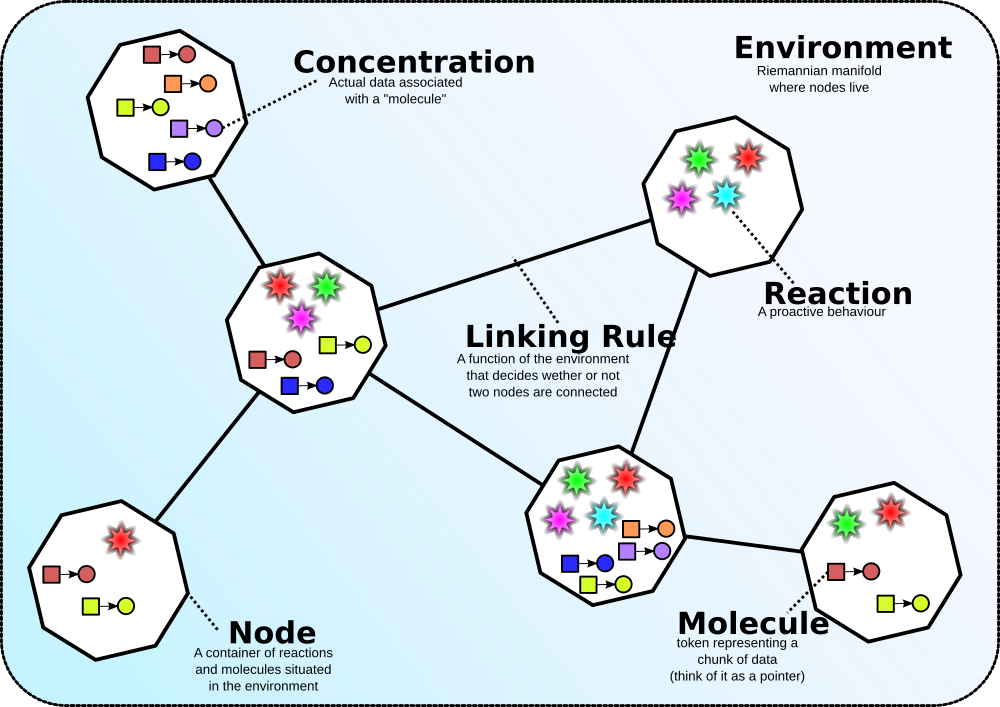
\includegraphics[width=12.5cm]{images/model.png} % inserisce una figura larga 12.5cm
% inserisce la legenda ed etichetta la figura con \label{fig:prima}
\caption[Illustrazione meta-modello di Alchemist]{Illustrazione meta-modello di Alchemist} \label{fig:alchemistModel}
\end{center}
\end{figure}

L'\textbf{\textit{Environment}} \`e l'astrazione dello spazio ed \`e anche l'entit\`a pi\`u esterna che funge da contenitore per i \textit{nodi}. Conosce la posizione di ogni \textit{nodo} nello spazio ed \`e quindi in grado di fornire la distanza tra due di essi e ne permette inoltre lo spostamento.

\`E detta \textbf{\textit{Linking rule}} una funzione dello stato corrente dell'\textit{environment} che associa ad ogni \textit{nodo} un \textbf{\textit{Vicinato}}, il quale \`e un entit\`a composta dal \textit{nodo} e da un set di \textit{nodi}, i vicini.

Un \textbf{\textit{Nodo}} \`e un contenitore di \textit{molecole} e \textit{reazioni} che \`e posizinato all'interno di un \textit{environment}.

La \textbf{\textit{Molecola}} \`e il nome di un dato, paragonabile a quello che rappresenta il nome di una variabile per i linguaggi imperativi.
Il valore da associare ad una \textit{molecola} \`e detto \textbf{\textit{Concentrazione}}.

%crea l'ambiente figura;
\begin{figure}[h] % [h] sta per here, cioè la figura va qui
\begin{center} % centra nel mezzo della pagina la figura
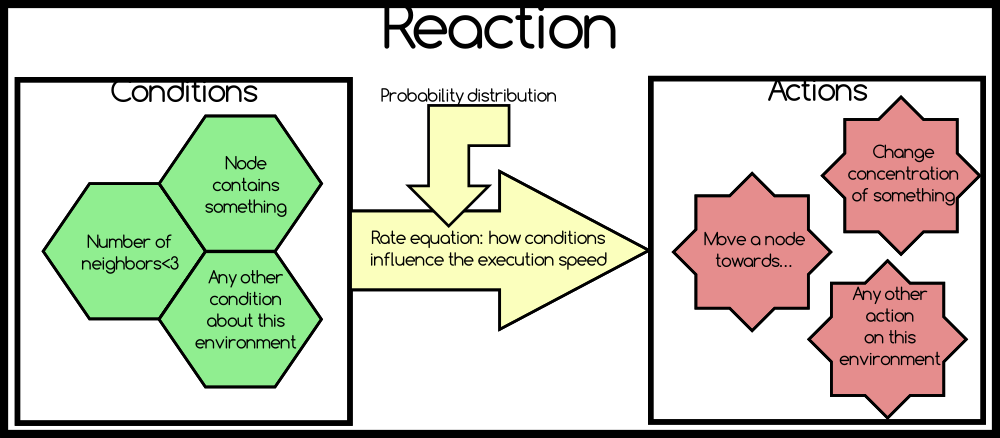
\includegraphics[width=14cm]{images/reaction.png} % inserisce una figura larga 12.5cm
% inserisce la legenda ed etichetta la figura con \label{fig:prima}
\caption[Illustrazione modello reazione di Alchemist]{Illustrazione modello reazione di Alchemist} \label{fig:alchemistReaction}
\end{center}
\end{figure}

Una \textbf{\textit{Reazione}} \`e un qualsiasi evento che pu\`o cambiare lo stato dell'\textit{environment} ed \`e. definita tramite una lista di \textit{condizioni}, una o pi\`u \textit{azioni} e una \textit{distribuzione temporale}.
\\La frequenza con cui avvengono dipende da:
\begin{itemize}
\item un parametro statico di frequenza;
\item il valore di ogni condizione;
\item un'equazione di frequenza che combina il tasso statico e il valore delle condizioni restituendo la frequenza istantanea;
\item una distribuzione temporale.
\end{itemize}
Ogni \textit{nodo} contiene un set di \textit{reazioni} che pu\`o essere anche vuoto.

Per comprendere meglio il meccanismo di una reazione si pu\`o osservare la figura \ref{fig:alchemistReaction}.

Una \textbf{\textit{Condizione}} \`e una funzione che prende come input l'\textit{environment} corrente e restituisce come output un booleano e un numero. Se la \textit{condizione} non si verifica, le \textit{azioni} associate a quella  \textit{reazione} non saranno eseguite. In relazione a parametri di configurazione e alla \textit{distribuzione temporale}, una \textit{condizione} potrebbe influire sulla velocit\`a della \textit{reazione}.

Un'\textbf{\textit{Azione}} \`e la definizione di una serie di operazioni che modellano un cambiamento nell'\textit{environment}.

In Alchemist un'incarnazione \`e un'istanza concreta del meta-modello appena descritta e che implementa una serie di componenti base come: la definizione di una molecola e del tipo di dati della concentrazione, un set di condizioni, le azioni e le reazioni. Incarnazioni diverse possono modellare universi completamente differenti.

%++-++-++-++-++-++-++-++-++-++-++-++-++-++-++-++-++-++-++-++-++-++-++-++-++-++-
\section{Scrivere una simulazione}

%-%-%-%-%-%-%-%-%-%-%-%-%-%-%-%-%-%-%-%-%-%-%-%-%-%-%-%-%-%-%-%-%-%-%-%-%-%-%-%-
\chapter{Agenti}
% imposta l'intestazione di pagina
\lhead[\fancyplain{}{\bfseries\thepage}]{\fancyplain{}{\bfseries\rightmark}}
% mette i numeri arabi
\pagenumbering{arabic}
Un'agente \`e un entit\`a che agisce in modo autonomo e continuo in uno spazio condiviso con altri agenti. Le caratteristiche principali di un agente sono: autonomia, proattivit\`a e reattivit\`a. Gli agenti sono formati da un nome, che \`e una caratteristica statica, e da componenti dinamici come lo stato.

%++-++-++-++-++-++-++-++-++-++-++-++-++-++-++-++-++-++-++-++-++-++-++-++-++-++-
\section{Agenti BDI}
Gli agenti BDI forniscono un meccanismo per separare le attivit\`a di selezione di un piano, presente nella lista dei piani, dall'esecuzione del piano attivo e quindi permettono di bilanciare il tempo speso nella scelta del piano e quello per eseguirlo.

I \textbf{\textit{Beliefs}} sono informazioni dello stato dell'agente, ovvero quello che lui sa del mondo (di se stesso e degli altri agenti), e possono comprendere regole di inferenza per permettere l'aggiunta di nuovi \textit{belief}.
\\Inoltre si possono modificare nel tempo: l'insieme dei \textit{belief} di un agente \`e dettto 'belief base' o 'belief set'.

I \textbf{\textit{Desires}} sono tutti i possibili piani che l'agente potrebbe eseguire. Rappresentano gli obiettivi o le situazioni che l'agente vorrebbe realizzare o portare a termine. I \textit{goals} sono \textit{desires} che l'agente persegue attivamente: per questo motivo, in generale, i piani desiderabili possono non essere coerenti tra loro mentre i \textit{goals} \`e bene che lo siano.

I \textbf{\textit{Intentions}} sono piani a cui l'agente ha deciso di lavorare o a cui sta gi\`a lavorando. I piani sono sequenze di azioni che un agente pu\`o eseguire per raggiungere un'\textit{intention} e a loro volta ne possono includere altri.

Gli \textbf{\textit{Eventi}} innescano le attivit\`a reattive degli agenti il cui risultato pu\`o essere l'aggiornamento dei \textit{beliefs}, la chiamata ad altri piani o la modifica di \textit{goals}.

Il ciclo di ragionamento di un agente avviene come descritto in figura \ref{fig:reasoningCicle}.
%crea l'ambiente figura;
\begin{figure}[h] % [h] sta per here, cioè la figura va qui
\begin{center} % centra nel mezzo della pagina la figura
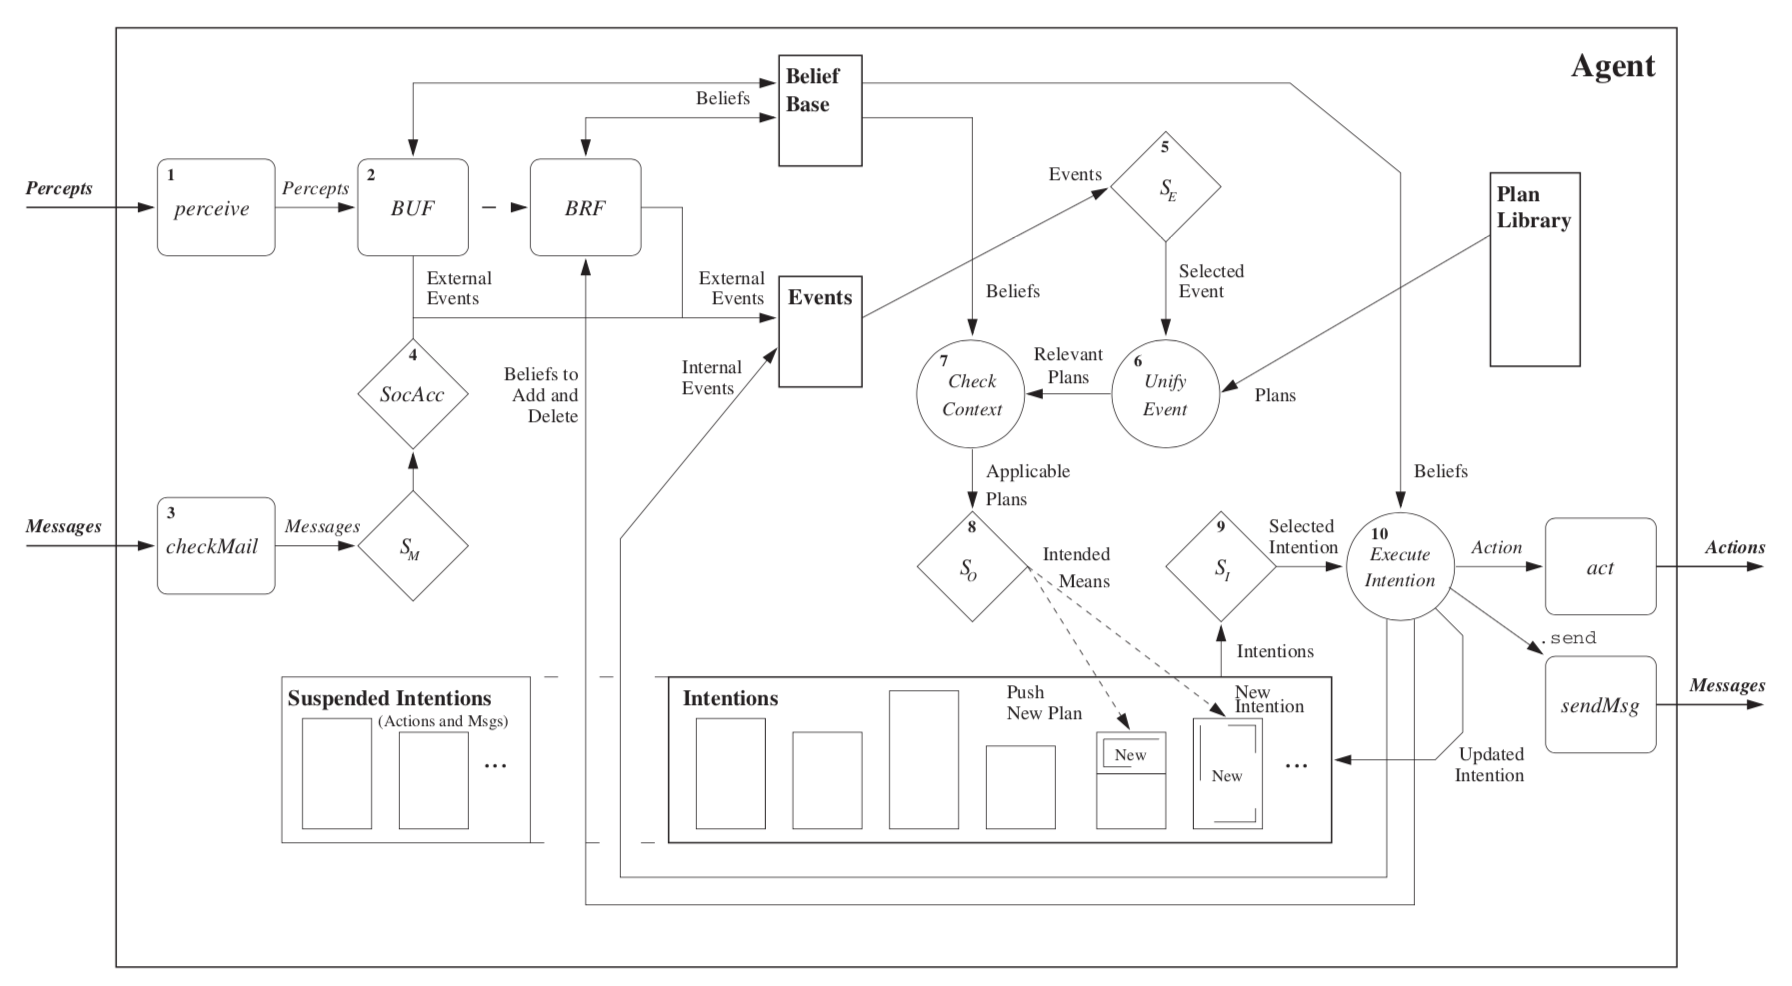
\includegraphics[width=16cm]{images/reasoningCicle.png} % inserisce una figura larga 12.5cm
% inserisce la legenda ed etichetta la figura con \label{fig:prima}
\caption[Ciclo di ragionamento di un agente]{Ciclo di ragionamento di un agente} \label{fig:reasoningCicle}
\end{center}
\end{figure}


%++-++-++-++-++-++-++-++-++-++-++-++-++-++-++-++-++-++-++-++-++-++-++-++-++-++-
\section{Ciclo di ragionamento}
RIVEDERE IL PEZZO QUI SOTTO E CONTINUARLO....
\\
\\
\\
La prima cosa che fa un agente nel ciclo di ragionamento \`e controllare l'ambiente per aggiornare i \textit{beliefs} con lo stato attuale. Quindi \`e necessario che l'agente abbia dei componenti per percepire i cambiamenti dell'ambiente. Una volta ottenuta la lista dei cambiamenti percepiti \`e necessario aggiornare la \textit{belief base} (che contiene l'insieme dei \textit{beliefs} dell'utente allo stato attuale).
\\
\\
// TODO CONTINUARE la descrizione del ciclo di ragionamento dell'agente....
% Modello ad agenti (JASON)
% Il funzionamento di un agente (reasoning cicle) prevede le seguenti fasi:
% - percezione di un cambiamento nell’environment e aggiornamento dei belief in base ai percepts ottenuti
% - ricezione di messaggi da parte di altri agenti e selezione dei messaggi accettabili
% - selezione di un evento tra quelli presenti nel set di quelli pending tramite politica FIFO
% - scelta dei piani rilevanti (dal set di piani della libreria) in base all’evento corrente e, quindi, selezione (dal set di piani rilevanti) di quelli applicabili in base al contesto dell’agente
% - selezione di un piano che verrà inserito nel set di intention dell’agente
% - selezione e esecuzione dell’intention da eseguire
% - se vi sono risposte disponibili, l’interprete inserisce le intention rilevanti nel set per permetterne la scelta nel prossimo ciclo
%
% Ad ogni ciclo vengono presi solamente un percept/messaggio, scelto un singolo evento (se disponibile) e successivamente eseguita una singola intention del piano selezionato.
% Le parti in cui l’agente deve scegliere quale messaggio/evento/piano/intention utilizzare possono essere riprogrammate per definire per ogni agente una priorità nella selezione.
%
%
% RIVEDERE
%  selezione del plan da inserire nelle intentions va in base all’ordine dei pian nella plan library


%-%-%-%-%-%-%-%-%-%-%-%-%-%-%-%-%-%-%-%-%-%-%-%-%-%-%-%-%-%-%-%-%-%-%-%-%-%-%-%-
\chapter{Progetto}
% imposta l'intestazione di pagina
\lhead[\fancyplain{}{\bfseries\thepage}]{\fancyplain{}{\bfseries\rightmark}}
% mette i numeri arabi
\pagenumbering{arabic}
Il progetto, come descritto nell'introduzione, ha come obiettivo l'implementazione del meta-modello di Alchemist attraverso la definizione di un incarnazione che modelli gli agenti all'interno del simulatore.

\section{Mapping dei modelli}
Il primo passo nell'evoluzione del progetto \`e stata l'analisi del mapping tra i due modelli, necessaria per individuare eventuali incongruenze o evidenziare opportunit\`a a livello applicativo, maggiore espressivit\`a.
Nei mapping effettuati si \`e cercato quindi di individuare l'entit\`a del meta-modello di Alchemist che offrisse maggiori opportunit\`a espressive per la definizione dell'agente.

Nella prima prova, l'agente \`e stato rapportato ad un nodo da cui ne deriva che l'environment sar\`a lo spazio che conterr\`a tutti gli agenti mentre, internamente al nodo, le molecole e le concentrazioni saranno utilizzate per gestire i beliefs dell'agente e le reazioni che saranno riferite ai piani utilizzando le condizioni come clausola per far scattare le azioni.
\\Questo tipo di mapping consentirebbe di realizzare simulazioni di sistemi non complessi in cui vi \`e un solo 'livello' di agenti che interagiscono tra loro. Questa affermazione pu\`o essere compresa meglio analizzando il secondo tentativo che \`e stato effettuato.

Nel secondo mapping, l'agente \`e stato spostato pi\`u internamente al nodo, in modo da far diventare il nodo stesso uno spazio per gli agenti che sono quindi mappati come reazioni. In questo modo l'environment sar\`a uno spazio in cui possono essere presenti pi\`u nodi, i quali a loro volta potranno contenere uno o pi\`u agenti. La frequenza con cui gli eventi sono innescati dipende, oltre che dai parametri passati nella configurazione della simulazione, anche dalle condizioni definite per quello specifico agente.
\\In questo caso si riuscir\`a a creare un sistema con pi\`u agenti all'interno di un singolo nodo, che in ambito applicativo pu\`o essere riferito ad un device, e che si muover\`a nello spazio insieme ad altri nodi, che conterranno altri agenti.

\section{Fasi di sviluppo}
Il passo successivo \`e stato quello di stilare un piano di sviluppo per affrontare il problema attraverso step incrementali. Questa scelta \`e stata dettata anche dalla poca conoscenza iniziale per lo sviluppo in Alchemist. Le fasi in cui \`e stato suddiviso il progetto sono state le seguenti:
\begin{enumerate}
\item Esecuzione di un'istruzione elementare da parte di un agente (ad esempio contatore);
\item Scambio di messaggi tra due agenti (ad esempio ping pong): inizialmente gli agenti possono anche risiedere nello stesso nodo ma poi l'implementazione deve prevedere il posizionamento degli agenti su nodi diversi;
\item Gestione del flusso di controllo attraverso l'inserimento di un operazione (come lo spostamento del nodo o l'incremento di un contatore) prima di effettuare la risposta al messaggio;
\item Gestione del flusso condizionato inserendo una clausola per la quale lo scambio di messaggi debba avvenire o meno.
\end{enumerate}


\section{Implementazioni}
% Definizione regole per stilizzazzione source code
\lstset{
tabsize = 2, %% Sets tab space width.
showstringspaces = false, %% Prevents space marking in strings, string is defined as the text that is generally printed directly to the console.
numbers = left, %% Displays line numbers on the left.
commentstyle = \color{green}, %% Sets comment color.
keywordstyle = \color{blue}, %% Sets  keyword color.
stringstyle = \color{red}, %% Sets  string color.
rulecolor = \color{black}, %% Sets frame color to avoid being affected by text color.
basicstyle = \small \ttfamily , %% Sets listing font and size.
breaklines = true, %% Enables line breaking.
numberstyle = \tiny,
}

Dopo aver esaminato i due modelli e aver analizzato i mapping realizzati si \`e deciso di implementare il caso che mappa l'agente alla reazione poich\`e seguendo lo schema del meta-modello di Alchemist l'implementazione risulta pi\`u immediata e espressiva.

\subsection{Scambio di messaggi tra agenti}
Lo sviluppo \`e partito dalla definizione della classe \textbf{AgentIncarnation} che implementa l'interfaccia Incarnation. I metodi definiti nell'interfaccia consentono di caratterizzare l'incarnazione nella creazione delle varie entit\`a del modello (nodi, distribuzioni temporali, reazioni, condizioni, azioni).

Per la creazione del nodo si \`e definita la classe \textbf{AgentsContainerNode} che estende AbstractNode. Questa classe ha tra le sue propriet\`a il riferiemnto all'environment in cui si trova il nodo e una struttura dati composta da coppie chiave e valore in cui la chiave \`e il nome dell'agente e il valore \`e il riferimento all'azione dell'agente.
% \\All'interno del nodo \`e presente un metodo che verr\`a invocato solamente dall'agente 'postman'

La distribuzione temporale di ogni reazione \`e stata realizzata istanziando la classe \textbf{DiracComb} inizializzata con il parametro recuperato dal file di configurazione della simulazione. La classe permette di emettere eventi ad un intervallo temporale specificato dal parametro passato.

Per le reazioni \`e stata definita la classe \textbf{AgentReaction} che rappresenta l'agente e che contiene le condizioni che devono verificarsi per far avvenire le azioni associate ad essa. Come propriet\`a della classe \`e presente solo una stringa che memorizza il nome dell'agente.
\\La creazione delle condizioni, per la fase iniziale del progetto, \`e stata fatta istanziando la classe \textbf{AbstractCondition} e implementando i metodi rimasti dell'interfaccia Condition: \textit{getContext} (definisce la profondit\`a della condizione GLOBAL,LOCAL,NEIGHBORHOOD), \textit{getPropensityContribution} (permette di influenzare la velocità della reazione che decide se utilizzare o meno questo parametro), \textit{isValid} (definisce la clausola per la valit\`a della condizione)).
\\L'azione da creare, ovvero il ciclo di ragionamento dell'agente, \`e passata della reazione come parametro. Per la prima fase, che prevedee un semplice scambio di messaggi, sono state definite le classi \textbf{SimpleAgentAction} e \textbf{PostmanAction} che estende la precedente. La prima ha come proprietà il nome dell'agente, un flag per l'inizializzazione, una mailbox formata da due code (una per la posta in entrata e una per quella in uscita) e un motore tuProlog. Al suo interno sono implementati i metodi \textit{execute} (che \`e il metodo principale in cui avviene il ciclo di ragionamento) e i metodi per la gestione delle caselle dei messaggi, le cui strutture sono definite come classi innestate InMessage e OutMessage rispettivamente per i messagggi in entrata e in uscita.
\\La classe \textbf{PostmanAction} sovrascrive l'implementazione del metodo \textit{execute} per invocare, ad ogni evento invocato dal simulatore, un metodo nel nodo che provveder\`a a prelevare i messaggi in uscita da ogni agente e recapitarli ai corretti destinatari.




%\begin{lstlisting}[language = Java , frame = trBL , firstnumber = last , escapeinside={(*@}{@*)}]
% public Node<Object> createNode(
%   final RandomGenerator rand,
%   final Environment<Object,P> env,
%   final String param) {
%     final Node<Object> node =
%       new AgentsContainerNode(param,
%         (Environment<Object, Position<? extends Continuous2DEnvironment>>) env);
%     return node;
% }
%\end{lstlisting}





% \clearpage{\pagestyle{empty}\cleardoublepage} % vedere se serve
\begin{thebibliography}{90} % crea l'ambiente bibliografia
\rhead[\fancyplain{}{\bfseries \leftmark}]{\fancyplain{}{\bfseries \thepage}}
\addcontentsline{toc}{chapter}{Bibliografia} % aggiunge la voce Bibliografia nell'indice

% provare anche questo comando:
\addcontentsline{toc}{chapter}{\numberline{}{Bibliografia}}
\bibitem{K1} alchemistsimulator.github.io
\bibitem{K2} Programming Multi-Agent Systems in AgentSpeak using Jason, (Rafael H. Bordini, Jomi Fred H\"{u}bner, Michael Wooldridge), Wiley, Interscience (2007)

% \bibitem{K3} Terzo oggetto bibliografia.
% \bibitem{K4} Quarto oggetto bibliografia.
\end{thebibliography}
\end{document}
